\documentclass[10pt,journal,compsoc,onecolumn]{IEEEtran}
\usepackage[utf8]{inputenc}
\usepackage{amsmath,amsfonts,amssymb}
\usepackage{amsthm}
\usepackage{graphicx}
\usepackage{cite}
\usepackage{textcomp}
\usepackage{tikz}
\usetikzlibrary{arrows,positioning,shapes.geometric}
\usepackage{booktabs}
\usepackage{url}
\usepackage{listings}
\usepackage{xcolor}
\usetikzlibrary{arrows,arrows.meta,positioning,shapes.geometric,calc,fit}

\definecolor{javagreen}{rgb}{0,0.5,0}
\definecolor{javagray}{rgb}{0.4,0.4,0.4}
\definecolor{javapurple}{rgb}{0.5,0,0.7}
\definecolor{backcolour}{rgb}{0.97,0.97,0.97}
\definecolor{javablue}{rgb}{0.0,0.2,0.7}

\lstdefinestyle{javastyle}{
    backgroundcolor=\color{backcolour},   
    commentstyle=\color{javagreen}\itshape,
    keywordstyle=\color{javablue}\bfseries,
    numberstyle=\tiny\color{javagray},
    stringstyle=\color{javapurple},
    basicstyle=\ttfamily\footnotesize,
    breakatwhitespace=false,         
    breaklines=true,                 
    captionpos=b,                    
    keepspaces=true,                 
    numbers=left,                    
    numbersep=5pt,                  
    showspaces=false,                
    showstringspaces=false,
    showtabs=false,                  
    tabsize=2,
    frame=single,
    rulecolor=\color{black!20}
}
\lstset{style=javastyle}

\newtheorem{theorem}{Theorem}
\newtheorem{lemma}[theorem]{Lemma}
\newtheorem{definition}[theorem]{Definition}
\newtheorem{corollary}[theorem]{Corollary}

\begin{document}

\title{Comprehensive Formalization and Algorithmic Taxonomy of Contiguous Subarray Problems: Prefix State Hashing, Sliding Window Invariants, AtMost Duality, Kadane Dynamic Programming, Monotonic Stacks, and Bitwise Monotonicity}

\IEEEtitleabstractindextext{%
\begin{abstract}
Contiguous subarray problems form a fundamental computational primitive across sequence optimization, dynamic programming, and technical coding platforms such as LeetCode. A central challenge in sequence processing is evaluating metrics---such as sum, product, parity, distinct element counts, minimums, maximums, or bitwise combinations---over bounded contiguous segments. Naive brute-force enumeration evaluates quadratic $\mathcal{O}(N^2)$ candidate windows, incurring $\mathcal{O}(N^3)$ time. This research paper presents an exhaustive, publication-grade taxonomy and algorithmic analysis of contiguous subarray problems. We establish eight foundational paradigms that systematically govern all optimal solutions: (1) Prefix-Sum Space and Hash-Map Equivalence Classes ($\mathcal{O}(N)$ exact sum, remainder, and zero-sum balance matching), (2) Two-Pointer Sliding Window Contractions ($\mathcal{O}(N)$ greedy optimization on monotonic non-negative domains), (3) The AtMost(K) Set-Theoretic Duality (Exact-$K$ count decomposition via inclusion-exclusion), (4) Dynamic Programming \& Kadane's Local State Optimization ($\mathcal{O}(N)$ maximum, minimum, and product subarray state transitions and circular topologies), (5) Monotonic Stack \& Element Contribution Mechanics ($\mathcal{O}(N)$ range boundaries, sum of subarray minimums, and min-products), (6) Sliding Window with Monotonic Extremum Queues ($\mathcal{O}(1)$ amortized window min/max bounds), (7) Non-Monotonic Prefix Spaces with Inequalities ($\mathcal{O}(N \log N)$ merge sort divide-and-conquer and $\mathcal{O}(N)$ monotonic deques on prefix sums), and (8) Bitwise Monotonicity \& Bounded State Transitions ($\mathcal{O}(30N)$ accumulation limits for OR and AND). For each paradigm, we present mathematical invariant proofs, complexity theorems, edge-case taxons, vector TikZ architectural diagrams, complete compilable Java reference implementations, and synthesize a 10-second diagnostic decision flowchart and master LeetCode taxonomy matrix.
\end{abstract}

\begin{IEEEkeywords}
Contiguous Subarrays, LeetCode Patterns, Prefix Sum Hashing, Sliding Window, AtMost Duality, Kadane Algorithm, Monotonic Stack, Element Contribution Principle, Monotonic Deque, Bitwise Monotonicity, Divide and Conquer
\end{IEEEkeywords}
}

\maketitle
\IEEEdisplaynontitleabstractindextext
\IEEEpeerreviewmaketitle

\section{Introduction and Mathematical Foundations}
\label{sec:intro}

Contiguous subarray problems represent a foundational computational primitive in algorithm design, data structures, dynamic programming, and competitive programming platforms such as LeetCode. A central challenge in sequence processing is evaluating metrics---such as sum, product, parity, distinct element counts, minimums, maximums, or bitwise combinations---over bounded contiguous segments of an array.

While brute-force enumeration of all candidate subarrays requires quadratic $\mathcal{O}(N^2)$ candidate evaluations and $\mathcal{O}(N^3)$ naive computation time, optimal algorithms achieve linear $\mathcal{O}(N)$ or linearithmic $\mathcal{O}(N \log N)$ execution time by exploiting structural invariants, algebraic equivalences, monotonic state transitions, and memory-efficient data structures.

This research paper presents an exhaustive, publication-grade taxonomy and algorithmic analysis of contiguous subarray problems. We establish eight fundamental paradigms that completely govern the design of optimal subarray algorithms for LeetCode:
\begin{enumerate}
    \item \textbf{Prefix-Sum Space and Hash-Map Equivalence Classes (\S\ref{sec:prefix-hash}):} Decomposing contiguous subarray metrics into prefix state differences, enabling exact sum matching, divisibility classes, zero-sum optimizations, and domain transformations in $\mathcal{O}(N)$ time.
    \item \textbf{Sliding Window and Two-Pointer Search Space Pruning (\S\ref{sec:sliding-window}):} Exploiting monotonic contraction properties across non-negative domains to prune candidate states from $\mathcal{O}(N^2)$ to $\mathcal{O}(N)$, including fixed-window and variable-window metrics.
    \item \textbf{The AtMost(K) Set-Theoretic Duality (\S\ref{sec:atmost-duality}):} Solving exact-$K$ count constraints over non-monotonic cardinality boundaries via set-theoretic decomposition: $\text{Exact}(K) = \text{AtMost}(K) - \text{AtMost}(K-1)$.
    \item \textbf{Dynamic Programming and Kadane's Local State Optimization (\S\ref{sec:dynamic-programming}):} Formalizing optimal sub-structure for maximum/minimum subarray sums, product propagation under multiplicative sign inversion, circular topology transformations, and single-element deletion models.
    \item \textbf{Monotonic Stack and Element Contribution Mechanics (\S\ref{sec:monotonic-stack}):} Inverting search focus from subarray iteration to element contribution, deriving exact left/right boundary ranges ($PSE$ and $NSE$) to evaluate sum of subarray minimums, maximums, and min-products in $\mathcal{O}(N)$ time.
    \item \textbf{Sliding Window with Monotonic Extremum Queues (\S\ref{sec:monotonic-queues}):} Tracking running window minimums and maximums in $\mathcal{O}(1)$ amortized time via monotonic double-ended queues.
    \item \textbf{Divide-and-Conquer, Range Trees, and Monotonic Deques on Negative Prefixes (\S\ref{sec:divide-conquer}):} Resolving non-monotonic prefix spaces for range sum bounds ($\mathcal{O}(N \log N)$ merge-sort divide and conquer) and shortest target sums with negative numbers ($\mathcal{O}(N)$ monotonic deque on prefix sums).
    \item \textbf{Bitwise Monotonicity and Bounded State Transitions (\S\ref{sec:bitwise}):} Exploiting the 32-bit accumulation boundary of bitwise OR and AND operations to constrain distinct subarray bitwise states to $\mathcal{O}(30 N)$.
\end{enumerate}

Furthermore, we provide complete, compilable Java reference implementations for every canonical problem class, formal mathematical proofs of invariant correctness, high-resolution vector TikZ architectural diagrams, and synthesize a diagnostic decision tree and taxonomy matrix (\S\ref{sec:taxonomy}) for immediate classification of any LeetCode subarray problem.

\subsection{Formal Definitions and Notation}

Let $A = [a_0, a_1, \dots, a_{N-1}]$ be a sequence of $N$ real or integer elements indexed from $0$ to $N-1$.

\begin{definition}[Contiguous Subarray]
A contiguous subarray $A[i \dots j]$ defined by start boundary $i$ and end boundary $j$ (where $0 \le i \le j < N$) is the ordered subsequence of elements:
\begin{equation}
A[i \dots j] = (a_i, a_{i+1}, \dots, a_j)
\end{equation}
A subarray is strictly contiguous: no elements within $[i, j]$ may be omitted, preserving spatial locality.
\end{definition}

\begin{theorem}[Cardinality of Subarray Space]
The total number of non-empty contiguous subarrays in an array of size $N$ is exactly $\frac{N(N+1)}{2} = \mathcal{O}(N^2)$.
\end{theorem}
\begin{proof}
A contiguous subarray is uniquely identified by choosing a pair of indices $(i, j)$ such that $0 \le i \le j < N$. Summing the number of valid ending indices $j$ for each starting index $i$:
\begin{equation}
\sum_{i=0}^{N-1} (N - i) = N + (N-1) + \dots + 1 = \frac{N(N+1)}{2} = \frac{N^2 + N}{2} = \mathcal{O}(N^2)
\end{equation}
\end{proof}

\begin{definition}[Subarray vs. Subsequence vs. Subset]
It is critical to distinguish these three structural concepts:
\begin{itemize}
    \item \textbf{Subarray}: Elements must be contiguous and in original order ($2^{\mathcal{O}(\log N)}$ cardinality, $\frac{N(N+1)}{2}$ candidates).
    \item \textbf{Subsequence}: Elements maintain relative order but can have arbitrary gaps ($2^N$ candidates).
    \item \textbf{Subset}: Elements can be chosen in arbitrary order without sequence preservation ($2^N$ candidates).
\end{itemize}
\end{definition}

\begin{theorem}[The Element Contribution Principle]
In the sum of all $\frac{N(N+1)}{2}$ contiguous subarrays, element $a_i$ (at index $i$, $0 \le i < N$) appears in exactly $(i + 1)(N - i)$ subarrays. Consequently:
\begin{equation}
\sum_{0 \le i \le j < N} \sum_{k=i}^{j} a_k = \sum_{i=0}^{N-1} (i + 1)(N - i) \cdot a_i
\end{equation}
\end{theorem}
\begin{proof}
A subarray $A[L \dots R]$ contains $a_i$ if and only if $L \le i$ and $R \ge i$. The number of valid left boundary choices is $i - 0 + 1 = i + 1$. The number of valid right boundary choices is $(N - 1) - i + 1 = N - i$. By the product rule of combinatorics, $a_i$ participates in exactly $(i + 1)(N - i)$ contiguous subarrays.
\end{proof}

\begin{definition}[Prefix Sum Array]
The prefix sum array $P$ of sequence $A$ is defined for $r \in [0, N-1]$ as:
\begin{equation}
P[r] = \sum_{k=0}^{r} a_k \quad \text{with base definition } P[-1] = 0
\end{equation}
\end{definition}

\begin{lemma}[Subarray Sum Decomposition]
The sum of elements in contiguous subarray $A[i \dots j]$, denoted $S(i, j)$, equals the difference of prefix sums:
\begin{equation}
S(i, j) = \sum_{k=i}^{j} a_k = P[j] - P[i-1] \quad \text{for } 0 \le i \le j < N
\end{equation}
\end{lemma}

%% ============================================================
\section{Paradigm 1: Prefix-Sum Space and Hash-Map Equivalence Classes}
\label{sec:prefix-hash}

The algebraic identity $S(i, j) = P[j] - P[i-1]$ allows us to recast the search for contiguous subarrays into an equivalent two-sum lookup on prefix sums: finding $i$ such that $P[i-1] = P[j] - K$.

\subsection{Why Sliding Window Fails on Negative Numbers}
A classic interview pitfall is attempting to solve subarray sum problems involving negative integers using two-pointer sliding windows. A two-pointer sliding window strictly requires \textbf{monotonicity}: advancing the right pointer must monotonically increase (or decrease) the window metric, and advancing the left pointer must monotonically invert that change. When negative numbers are present, adding an element can either increase or decrease the sum, destroying monotonicity and invalidating greedy window contractions. Prefix sum hashing is the exact remedy.

\subsection{Target Sum Matching ($P[j] - P[i-1] = K$)}

\subsubsection{Subarray Sum Equals K (LeetCode 560)}
We iterate $j$ from $0$ to $N-1$, maintaining cumulative running prefix $P[j]$ and a frequency hash map $M$. For each $j$, the number of subarrays ending at $j$ with sum $K$ equals the frequency of prefix value $(P[j] - K)$ observed prior to index $j$.
\begin{itemize}
    \item \textbf{Mandatory Base Case Guard}: $M[0] = 1$. This accounts for subarrays starting at index $0$ ($A[0 \dots j]$), where $P[j] = K \implies P[j] - K = 0 = P[-1]$. Omitting this base case silently drops all valid prefix subarrays starting at index 0.
\end{itemize}

\subsubsection{Maximum Size Subarray Sum Equals K (LeetCode 325)}
When seeking the \emph{maximum length} of a subarray with sum $K$, the hash map stores the \textbf{earliest occurrence index} of each prefix sum: $M[P[i-1]] = i - 1$. Upon encountering $P[j]$, if $(P[j] - K) \in M$, candidate length is $j - M[P[j] - K]$. To maximize length, existing keys are never overwritten.

\subsection{Modulo and Remainder Equivalence Classes ($S(i, j) \pmod K = 0$)}

\subsubsection{Subarray Sums Divisible by K (LeetCode 974)}
By number theory, $S(i, j) \equiv 0 \pmod K \iff P[j] \equiv P[i-1] \pmod K$.
Thus, any two prefix sums sharing the same remainder modulo $K$ delineate a contiguous subarray whose sum is an exact multiple of $K$.
\begin{itemize}
    \item \textbf{The Negative Modulo Trap in Java}: In Java, the modulo operator \texttt{\%} retains the sign of the dividend (e.g., \texttt{-7 \% 5 = -2}). In modular arithmetic, remainders must reside in $[0, K-1]$. The normalized positive remainder is:
    \begin{equation}
    rem = ((pref \pmod K) + K) \pmod K
    \end{equation}
\end{itemize}

\subsubsection{Continuous Subarray Sum of Length at Least 2 (LeetCode 523)}
Requires $S(i, j) = m \cdot K$ and length $(j - i + 1) \ge 2$. We store the earliest index of each remainder in a hash map initialized with $M[0] = -1$. When $rem$ is seen again at index $j$, if $j - M[rem] \ge 2$, return true.

\subsection{Domain Transformation: Equal 0s and 1s \& Parity Matching}

\subsubsection{Contiguous Array with Equal 0s and 1s (LeetCode 525)}
Transform the binary array into balance space by mapping $0 \to -1$ and $1 \to +1$. A subarray has equal 0s and 1s if and only if its transformed sum equals $0$. The problem reduces directly to finding the longest subarray with sum $0$ ($P[j] = P[i-1]$).

\subsubsection{Number of Subarrays with Odd Sum (LeetCode 1524)}
A sum is odd if and only if the parity of $P[j]$ differs from $P[i-1]$. We simply maintain running counts of even and odd prefix sums seen so far.

\subsection{Compilable Java Reference Implementations}

\begin{lstlisting}[language=Java]
import java.util.HashMap;
import java.util.Map;

public class PrefixHashSubarraySolutions {

    // 1. Subarray Sum Equals K (LeetCode 560) - O(N) Time, O(N) Space
    public static int subarraySumEqualsK(int[] nums, int k) {
        Map<Long, Integer> freq = new HashMap<>();
        freq.put(0L, 1); // Base case: P[-1] = 0
        long pref = 0;
        int count = 0;
        
        for (int x : nums) {
            pref += x;
            if (freq.containsKey(pref - k)) {
                count += freq.get(pref - k);
            }
            freq.put(pref, freq.getOrDefault(pref, 0) + 1);
        }
        return count;
    }

    // 2. Subarray Sums Divisible by K (LeetCode 974) - O(N) Time, O(K) Space
    public static int subarraysDivByK(int[] nums, int k) {
        int[] remFreq = new int[k];
        remFreq[0] = 1; // Base case: remainder 0 seen once at start
        long pref = 0;
        int count = 0;
        
        for (int x : nums) {
            pref += x;
            int rem = (int) ((pref % k + k) % k); // Positive normalized modulo
            count += remFreq[rem];
            remFreq[rem]++;
        }
        return count;
    }

    // 3. Contiguous Array - Equal 0s and 1s (LeetCode 525) - O(N) Time, O(N) Space
    public static int findMaxLengthEqual01(int[] nums) {
        Map<Integer, Integer> firstSeen = new HashMap<>();
        firstSeen.put(0, -1); // Base case: balance 0 at index -1
        int pref = 0;
        int maxLen = 0;
        
        for (int j = 0; j < nums.length; j++) {
            pref += (nums[j] == 1) ? 1 : -1;
            if (firstSeen.containsKey(pref)) {
                maxLen = Math.max(maxLen, j - firstSeen.get(pref));
            } else {
                firstSeen.put(pref, j); // Retain earliest index
            }
        }
        return maxLen;
    }
}
\end{lstlisting}

%% ============================================================
\section{Paradigm 2: Sliding Window and Two-Pointer Search Space Pruning}
\label{sec:sliding-window}

When sequence elements are strictly non-negative ($a_k \ge 0$), the prefix sum sequence $P[j]$ is monotonically non-decreasing ($P[j] \ge P[j-1]$). Expanding the right boundary $R$ increases window sum and distinct element counts, while advancing the left boundary $L$ decreases window metrics. This monotonicity enables two-pointer search space pruning from $\mathcal{O}(N^2)$ to amortized $\mathcal{O}(N)$.

\subsection{Fixed-Size Window Pattern}
When subarray length is constrained to an exact constant $K$, the window $[i, i + K - 1]$ maintains state by sliding: adding incoming element $a_{i+K-1}$ and dropping outgoing element $a_{i-1}$ in $\mathcal{O}(1)$ time.
\begin{itemize}
    \item \textbf{Maximum Average Subarray I (LeetCode 643)}: Running sum of length $K$.
    \item \textbf{Maximum Sum of Distinct Subarrays with Length K (LeetCode 2461)}: Frequency map/set alongside running sum, verifying $|set| == K$.
\end{itemize}

\subsection{Variable Window Contraction Mechanics}

\subsubsection{Minimum Size Subarray Sum (LeetCode 209)}
We maintain window $[L, R]$. For each $R$, we add $A[R]$ to $window\_sum$. While $window\_sum \ge Target$, we update $min\_len = \min(min\_len, R - L + 1)$ and contract $L$ by subtracting $A[L]$.

\begin{theorem}[Amortized Linear Complexity of Sliding Window]
The two-pointer sliding window algorithm executes in $\mathcal{O}(N)$ total time complexity and $\mathcal{O}(1)$ auxiliary space.
\end{theorem}
\begin{proof}
The right pointer $R$ increments from $0$ to $N-1$ exactly $N$ times. The left pointer $L$ increments monotonically from $0$ to $N-1$ and never decrements. Across the entire execution, $L$ is incremented at most $N$ times. Total pointer movements are bounded by $2N = \mathcal{O}(N)$.
\end{proof}

\subsubsection{Subarray Product Less Than K (LeetCode 713)}
For positive integer arrays, expanding $R$ multiplies $prod$ by $A[R]$. While $prod \ge K$, we divide $prod$ by $A[L]$ and advance $L$.
\begin{lemma}[Ending-At Count Invariant]
For a valid window $[L, R]$ where all sub-windows ending at $R$ satisfy the condition, the number of valid contiguous subarrays ending strictly at $R$ is exactly $R - L + 1$.
\end{lemma}
\begin{proof}
The valid subarrays ending at $R$ are $A[R \dots R], A[R-1 \dots R], \dots, A[L \dots R]$. The starting indices range from $L$ to $R$, giving $(R - L + 1)$ distinct choices.
\end{proof}

\subsection{Compilable Java Reference Implementations}

\begin{lstlisting}[language=Java]
public class SlidingWindowSubarraySolutions {

    // 1. Minimum Size Subarray Sum >= S (LeetCode 209) - O(N) Time, O(1) Space
    public static int minSubArrayLen(int target, int[] nums) {
        int L = 0, sum = 0, minLen = Integer.MAX_VALUE;
        for (int R = 0; R < nums.length; R++) {
            sum += nums[R];
            while (sum >= target) {
                minLen = Math.min(minLen, R - L + 1);
                sum -= nums[L++];
            }
        }
        return minLen == Integer.MAX_VALUE ? 0 : minLen;
    }

    // 2. Subarray Product Less Than K (LeetCode 713) - O(N) Time, O(1) Space
    public static int numSubarrayProductLessThanK(int[] nums, int k) {
        if (k <= 1) return 0;
        int L = 0, prod = 1, count = 0;
        for (int R = 0; R < nums.length; R++) {
            prod *= nums[R];
            while (prod >= k) {
                prod /= nums[L++];
            }
            count += (R - L + 1); // Ending-At Count Invariant
        }
        return count;
    }
}
\end{lstlisting}

%% ============================================================
\section{Paradigm 3: The AtMost(K) Set-Theoretic Duality}
\label{sec:atmost-duality}

A frequent obstacle in sequence optimization is counting contiguous subarrays satisfying an \textbf{exact} condition:
\begin{itemize}
    \item Subarrays with \emph{exactly} $K$ distinct integers (LeetCode 992).
    \item Binary subarrays with sum \emph{exactly} $K$ (LeetCode 930).
    \item Nice subarrays with \emph{exactly} $K$ odd integers (LeetCode 1248).
\end{itemize}

\subsection{Why Direct Sliding Window Fails for Exact K}
In sliding window algorithms, we require monotonic contraction: if a window satisfies a property, shrinking it preserves or drives it toward a boundary. However, the condition $|Distinct(A[L \dots R])| == K$ is \textbf{non-monotonic}. If a window has $K$ distinct elements, shrinking $L$ might either keep it at $K$ (if $A[L]$ occurs elsewhere in the window) or drop it to $K-1$. The left pointer cannot greedily advance without potentially skipping valid sub-windows.

\subsection{The Master Set Duality Formula}
By basic set theory, the set of subarrays satisfying an exact metric $K$ equals the set difference between those satisfying $\le K$ and those satisfying $\le (K - 1)$:
\begin{equation}
\text{Exact}(K) = \text{AtMost}(K) - \text{AtMost}(K - 1)
\end{equation}

\begin{figure}[htbp]
\centering
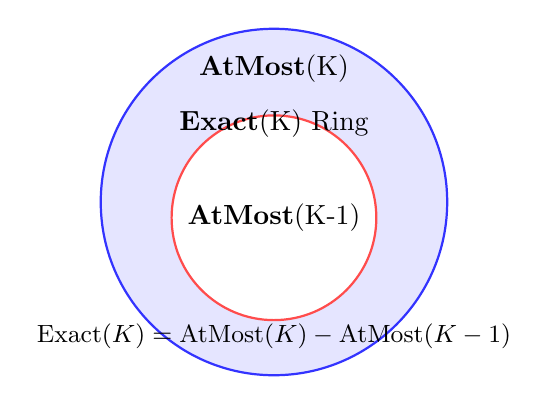
\begin{tikzpicture}[
    venn/.style={draw, circle, thick, align=center},
    arr/.style={->, >=stealth, thick, color=blue!70!black}
]
    % Outer Circle (AtMost K)
    \draw[fill=blue!10, draw=blue!80, thick] (0,0) circle (2.2cm);
    \node at (0, 1.7) {\textbf{AtMost}(K)};
    
    % Inner Circle (AtMost K-1)
    \draw[fill=white, draw=red!70, thick] (0,-0.2) circle (1.3cm);
    \node at (0, -0.2) {\textbf{AtMost}(K-1)};
    
    % Shaded Difference
    \node at (0, 1.0) {\textbf{Exact}(K) Ring};
    \node at (0, -1.7) {\small $\text{Exact}(K) = \text{AtMost}(K) - \text{AtMost}(K-1)$};
\end{tikzpicture}
\caption{The Set-Theoretic Duality for Exact-$K$ Subarrays. Calculating $\text{AtMost}(K)$ is monotonic and solvable in $\mathcal{O}(N)$ sliding window time.}
\label{fig:atmost_venn}
\end{figure}

The condition $\text{AtMost}(K)$ is \textbf{strictly monotonic}: as $R$ expands, distinct count or sum increases; as $L$ contracts, it decreases. Thus, $\text{AtMost}(K)$ can be evaluated in pure $\mathcal{O}(N)$ time. Evaluating it twice ($\text{AtMost}(K)$ and $\text{AtMost}(K-1)$) yields the exact answer in $\mathcal{O}(N)$ time and $\mathcal{O}(1)$ space!

\subsection{Compilable Java Reference Implementation}

\begin{lstlisting}[language=Java]
import java.util.HashMap;
import java.util.Map;

public class AtMostDualitySolutions {

    // Subarrays with K Different Integers (LeetCode 992) - O(N) Time, O(K) Space
    public static int subarraysWithKDistinct(int[] nums, int k) {
        return atMostKDistinct(nums, k) - atMostKDistinct(nums, k - 1);
    }

    private static int atMostKDistinct(int[] nums, int k) {
        if (k <= 0) return 0;
        Map<Integer, Integer> freq = new HashMap<>();
        int L = 0, count = 0;
        
        for (int R = 0; R < nums.length; R++) {
            freq.put(nums[R], freq.getOrDefault(nums[R], 0) + 1);
            while (freq.size() > k) {
                freq.put(nums[L], freq.get(nums[L]) - 1);
                if (freq.get(nums[L]) == 0) freq.remove(nums[L]);
                L++;
            }
            count += (R - L + 1); // Subarrays ending at R with <= K distinct
        }
        return count;
    }
}
\end{lstlisting}

%% ============================================================
\section{Paradigm 4: Dynamic Programming and Kadane's Local State Optimization}
\label{sec:dynamic-programming}

Kadane's algorithm is the canonical dynamic programming framework for contiguous subarray optimization over real-valued sequences containing mixed positive and negative numbers.

\subsection{Classic Kadane's Algorithm (LeetCode 53)}
Let $dp[i]$ be the maximum subarray sum of any contiguous subarray ending \emph{strictly at index $i$}. At index $i$, we face an optimal decision:
\begin{enumerate}
    \item Extend the optimal subarray ending at $i-1$: $dp[i-1] + a_i$.
    \item Discard the historical sum and start a new subarray at $i$: $a_i$.
\end{enumerate}
\begin{equation}
dp[i] = \max(a_i, dp[i-1] + a_i)
\end{equation}
The global maximum is $\max_{0 \le i < N} dp[i]$. Since $dp[i]$ depends only on $dp[i-1]$, space collapses to $\mathcal{O}(1)$.

\subsubsection{Boundary Index Reconstruction}
To recover the start and end indices $[bestStart, bestEnd]$ of the maximum subarray:
\begin{lstlisting}[language=Java]
long currentSum = nums[0], maxSum = nums[0];
int bestStart = 0, bestEnd = 0, tempStart = 0;

for (int i = 1; i < nums.length; i++) {
    if (nums[i] > currentSum + nums[i]) {
        currentSum = nums[i]; // Start fresh
        tempStart = i;
    } else {
        currentSum += nums[i]; // Extend
    }
    if (currentSum > maxSum) {
        maxSum = currentSum;
        bestStart = tempStart;
        bestEnd = i;
    }
}
\end{lstlisting}

\subsection{Dual-State Propagation: Maximum Product Subarray (LeetCode 152)}
Multiplication by negative numbers inverts order ($\text{Negative} \times \text{Negative} = \text{Positive}$). A large negative product can instantly transform into the maximum positive product upon encountering another negative value.
\begin{itemize}
    \item \textbf{Dual State Recurrence}: Maintain both $currMax$ and $currMin$.
    \item \textbf{Negative Swap Invariant}: When $a_i < 0$, swap $currMax$ and $currMin$ before updating!
    \begin{align}
    currMax &= \max(a_i, currMax \cdot a_i) \\
    currMin &= \min(a_i, currMin \cdot a_i)
    \end{align}
\end{itemize}

\subsection{Circular Topology Transformations (LeetCode 918)}
In a circular array, a maximum subarray can either be:
\begin{enumerate}
    \item \textbf{Non-wrapping}: Resides within standard array boundaries $\implies KadaneMax$.
    \item \textbf{Wrapping}: Wraps across array boundary. Maximizing the elements at the ends is mathematically equivalent to \textbf{minimizing the elements left in the middle}:
    \begin{equation}
    WrappingMax = TotalSum - KadaneMin
    \end{equation}
\end{enumerate}
\begin{itemize}
    \item \textbf{The All-Negative Trap Guard}: If all numbers are negative, $TotalSum == KadaneMin$, causing $WrappingMax = 0$ (an empty subarray, which is disallowed). In this case, we must return $KadaneMax$.
\end{itemize}

\subsection{Subarray DP with Modifications (LeetCode 1186 \& 1749)}
\begin{itemize}
    \item \textbf{Maximum Subarray Sum with One Deletion (LeetCode 1186)}: Maintain $noDelete[i] = \max(a_i, noDelete[i-1] + a_i)$ and $oneDelete[i] = \max(noDelete[i-1], oneDelete[i-1] + a_i)$.
    \item \textbf{Maximum Absolute Sum of Any Subarray (LeetCode 1749)}: $\max(|S(i, j)|) = \max(P[j] - P[i-1]) = \max(P) - \min(P)$, computable in one single pass.
\end{itemize}

\subsection{Compilable Java Reference Implementations}

\begin{lstlisting}[language=Java]
public class KadaneSubarraySolutions {

    // 1. Maximum Product Subarray (LeetCode 152) - O(N) Time, O(1) Space
    public static int maxProduct(int[] nums) {
        long currMax = nums[0], currMin = nums[0], globalMax = nums[0];
        for (int i = 1; i < nums.length; i++) {
            if (nums[i] < 0) {
                long temp = currMax;
                currMax = currMin;
                currMin = temp; // Swap on negative
            }
            currMax = Math.max((long)nums[i], currMax * nums[i]);
            currMin = Math.min((long)nums[i], currMin * nums[i]);
            globalMax = Math.max(globalMax, currMax);
        }
        return (int) globalMax;
    }

    // 2. Maximum Sum Circular Subarray (LeetCode 918) - O(N) Time, O(1) Space
    public static int maxSubarraySumCircular(int[] nums) {
        int totalSum = 0;
        int currMax = 0, maxSum = nums[0];
        int currMin = 0, minSum = nums[0];

        for (int x : nums) {
            currMax = Math.max(x, currMax + x);
            maxSum = Math.max(maxSum, currMax);

            currMin = Math.min(x, currMin + x);
            minSum = Math.min(minSum, currMin);

            totalSum += x;
        }

        // All-Negative Trap Guard
        if (totalSum == minSum) return maxSum;
        return Math.max(maxSum, totalSum - minSum);
    }
}
\end{lstlisting}

%% ============================================================
\section{Paradigm 5: Monotonic Stack and Element Contribution Mechanics}
\label{sec:monotonic-stack}

A major class of LeetCode hard problems requires summing metrics over \emph{all possible subarrays}:
\begin{itemize}
    \item Sum of Subarray Minimums (LeetCode 907)
    \item Sum of Subarray Ranges (LeetCode 2104)
    \item Maximum Subarray Min-Product (LeetCode 1856)
\end{itemize}

Iterating all $\mathcal{O}(N^2)$ subarrays and finding minimums naively costs $\mathcal{O}(N^3)$ or $\mathcal{O}(N^2)$. The breakthrough algorithmic paradigm is \textbf{Element Contribution}: Inverting the question from ``What is the minimum of subarray $A[i \dots j]$?'' to:
\begin{center}
\emph{``In how many contiguous subarrays does element $A[i]$ act as the absolute minimum?''}
\end{center}

\subsection{Range Boundary Determination ($PSE$ and $NSE$)}
For each index $i$, element $A[i]$ remains the minimum in any subarray $A[L \dots R]$ as long as $A[i]$ is strictly smaller than all elements in that range:
\begin{itemize}
    \item \textbf{Previous Smaller Element ($PSE$)}: The closest index $L < i$ such that $A[L] < A[i]$.
    \item \textbf{Next Smaller Element ($NSE$)}: The closest index $R > i$ such that $A[R] \le A[i]$.
\end{itemize}

\begin{figure*}[htbp]
\centering
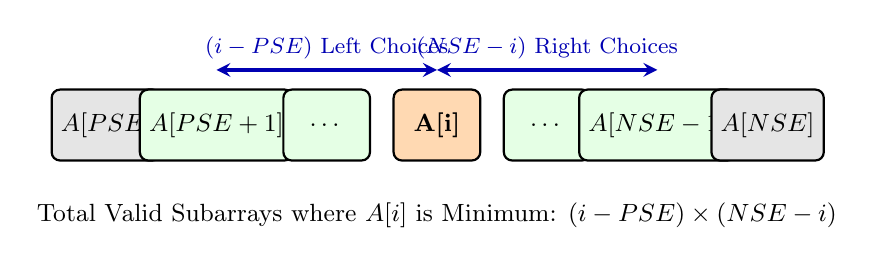
\begin{tikzpicture}[
    box/.style={draw, rectangle, rounded corners=3pt, thick, align=center, minimum width=1.1cm, minimum height=0.9cm, font=\small},
    spanarrow/.style={<->, >=stealth, very thick, color=blue!70!black}
]
    % Array Elements
    \node[box, fill=gray!20] (pse) at (0,0) {$A[PSE]$};
    \node[box, fill=green!10] (l1) at (1.4,0) {$A[PSE+1]$};
    \node[box, fill=green!10] (l2) at (2.8,0) {$\dots$};
    \node[box, fill=orange!30] (mid) at (4.2,0) {\textbf{A[i]}};
    \node[box, fill=green!10] (r1) at (5.6,0) {$\dots$};
    \node[box, fill=green!10] (r2) at (7.0,0) {$A[NSE-1]$};
    \node[box, fill=gray!20] (nse) at (8.4,0) {$A[NSE]$};
    
    % Span Annotations
    \draw[spanarrow] (1.4, 0.7) -- node[midway, above, font=\footnotesize] {$(i - PSE)$ Left Choices} (4.2, 0.7);
    \draw[spanarrow] (4.2, 0.7) -- node[midway, above, font=\footnotesize] {$(NSE - i)$ Right Choices} (7.0, 0.7);
    
    \node[below=0.4cm of mid, font=\small] {Total Valid Subarrays where $A[i]$ is Minimum: \textbf{$(i - PSE) \times (NSE - i)$}};
\end{tikzpicture}
\caption{The Element Contribution Span. Element $A[i]$ dominates as the minimum across all subarrays starting in $[PSE+1, i]$ and ending in $[i, NSE-1]$.}
\label{fig:element_contribution}
\end{figure*}

\begin{theorem}[Contribution Formula]
The total number of contiguous subarrays in which $A[i]$ is the minimum is exactly:
\begin{equation}
Count(i) = (i - PSE[i]) \times (NSE[i] - i)
\end{equation}
The total contribution of $A[i]$ to the sum of all subarray minimums is $A[i] \times Count(i)$.
\end{theorem}

\subsection{Duplicate Handling: Strict vs. Non-Strict Inequalities}
When duplicate elements exist (e.g., $[2, 4, 2]$), both $2$s could claim the subarray $[2, 4, 2]$ as their minimum, causing \textbf{double counting}.
\begin{itemize}
    \item \textbf{The Invariant Guard}: Define $PSE$ using \textbf{strict inequality} ($<$), and define $NSE$ using \textbf{non-strict inequality} ($\le$) (or vice versa).
    \item This partitions the subarray space into mutually exclusive and completely exhaustive sets, guaranteeing zero double-counting and zero missed subarrays.
\end{itemize}

\subsection{Compilable Java Reference Implementation}

\begin{lstlisting}[language=Java]
import java.util.ArrayDeque;
import java.util.Deque;

public class MonotonicStackSubarraySolutions {

    // Sum of Subarray Minimums (LeetCode 907) - O(N) Time, O(N) Space
    public static int sumSubarrayMins(int[] arr) {
        int N = arr.length;
        int MOD = 1_000_000_007;
        int[] pse = new int[N];
        int[] nse = new int[N];
        Deque<Integer> stack = new ArrayDeque<>();

        // Previous Smaller Element (Strictly Less <)
        for (int i = 0; i < N; i++) {
            while (!stack.isEmpty() && arr[stack.peek()] >= arr[i]) {
                stack.pop();
            }
            pse[i] = stack.isEmpty() ? -1 : stack.peek();
            stack.push(i);
        }

        stack.clear();

        // Next Smaller Element (Less Than or Equal <=)
        for (int i = N - 1; i >= 0; i--) {
            while (!stack.isEmpty() && arr[stack.peek()] > arr[i]) {
                stack.pop();
            }
            nse[i] = stack.isEmpty() ? N : stack.peek();
            stack.push(i);
        }

        // Aggregate Contributions
        long totalSum = 0;
        for (int i = 0; i < N; i++) {
            long leftChoices = i - pse[i];
            long rightChoices = nse[i] - i;
            long contribution = (leftChoices * rightChoices) % MOD;
            totalSum = (totalSum + contribution * arr[i]) % MOD;
        }
        return (int) totalSum;
    }

    // Maximum Subarray Min-Product (LeetCode 1856) - O(N) Time, O(N) Space
    public static int maxSumMinProduct(int[] nums) {
        int N = nums.length;
        long[] pref = new long[N + 1];
        for (int i = 0; i < N; i++) pref[i + 1] = pref[i] + nums[i];

        int[] pse = new int[N];
        int[] nse = new int[N];
        Deque<Integer> stack = new ArrayDeque<>();

        for (int i = 0; i < N; i++) {
            while (!stack.isEmpty() && nums[stack.peek()] >= nums[i]) stack.pop();
            pse[i] = stack.isEmpty() ? -1 : stack.peek();
            stack.push(i);
        }
        stack.clear();
        for (int i = N - 1; i >= 0; i--) {
            while (!stack.isEmpty() && nums[stack.peek()] >= nums[i]) stack.pop();
            nse[i] = stack.isEmpty() ? N : stack.peek();
            stack.push(i);
        }

        long maxProduct = 0;
        for (int i = 0; i < N; i++) {
            int L = pse[i] + 1;
            int R = nse[i] - 1;
            long sum = pref[R + 1] - pref[L];
            maxProduct = Math.max(maxProduct, sum * nums[i]);
        }
        return (int) (maxProduct % 1_000_000_007);
    }
}
\end{lstlisting}

%% ============================================================
\section{Paradigm 6: Sliding Window with Monotonic Extremum Queues}
\label{sec:monotonic-queues}

When maintaining running maximums or minimums inside a sliding window, standard priority queues incur $\mathcal{O}(N \log K)$ overhead. A Monotonic Double-Ended Queue (Deque) maintains indices whose values are strictly monotonic, enabling $\mathcal{O}(1)$ amortized queries.

\subsection{Sliding Window Maximum (LeetCode 239)}
We maintain a monotonic decreasing deque of indices. For incoming index $R$:
\begin{enumerate}
    \item Remove indices out of window bound: $dq.peek() \le R - K$.
    \item Maintain monotonicity: While $A[dq.peekLast()] \le A[R]$, pop back.
    \item Add $R$ to back. The maximum is always at $dq.peekFirst()$.
\end{enumerate}

\subsection{Continuous Subarray Absolute Difference Limit (LeetCode 1438)}
Maintain dual monotonic deques: one decreasing for window maximum, one increasing for window minimum. While $maxDq.first - minDq.first > Limit$, contract $L$.

%% ============================================================
\section{Paradigm 7: Non-Monotonic Prefix Spaces (Negative Numbers + Inequalities)}
\label{sec:divide-conquer}

When elements contain negative values and constraints involve \textbf{inequalities} (e.g., $S(i, j) \ge K$), prefix sums are non-monotonic, and standard hash maps cannot perform range queries. Two optimal paradigms resolve this space:

\subsection{Shortest Subarray with Sum at Least K (LeetCode 862)}
We construct prefix sums $P[j]$. We need $P[j] - P[i] \ge K$ with minimized $(j - i)$.
We maintain an increasing deque of prefix indices:
\begin{enumerate}
    \item \textbf{Check Target Invariant}: While $P[j] - P[dq.peekFirst()] \ge K$, record candidate length $j - dq.pollFirst()$. (Since $j$ increases, this $i$ can never yield a shorter subarray for any future $j' > j$).
    \item \textbf{Maintain Monotonicity}: While $P[j] \le P[dq.peekLast()]$, pop last (an index with higher prefix sum appearing earlier is strictly dominated by $j$).
\end{enumerate}
Complexity is amortized $\mathcal{O}(N)$ time and $\mathcal{O}(N)$ space!

\subsection{Count of Range Sums (LeetCode 327)}
Find the count of subarrays where $Lower \le S(i, j) \le Upper \iff Lower \le P[j] - P[i-1] \le Upper$.
This is solved in $\mathcal{O}(N \log N)$ time using Merge-Sort Divide-and-Conquer on prefix sums. During the merge step of sorted sub-arrays $[start, mid)$ and $[mid, end)$, for each $j \in [mid, end)$, we maintain two sliding pointers $[k_1, k_2)$ in the left half such that $P[j] - P[k] \in [Lower, Upper]$.

%% ============================================================
\section{Paradigm 8: Bitwise Monotonicity and Bounded State Transitions}
\label{sec:bitwise}

Bitwise operations over contiguous subarrays exhibit monotonicity properties that drastically limit state complexity.

\subsection{Bitwise OR Monotonicity (LeetCode 898 \& 2411)}
The bitwise OR operation is bit-accumulating: $A \text{ OR } B \ge A$. As window length increases, bits can only transition from $0 \to 1$ and never $1 \to 0$.

\begin{theorem}[30-Bit Monotonicity Bound]
In a 32-bit integer sequence, as left index $i$ moves from $j$ down to $0$, the cumulative bitwise OR value $A[i \dots j]$ can take at most 30 distinct values.
\end{theorem}
\begin{proof}
An integer has at most 30 value-bearing bits. Starting with $a_j$, extending leftwards can only set previously unset bit positions. Since set bits never clear, new distinct values occur only when at least one new bit is set to $1$. There are at most 30 available bits to set, bounding distinct OR values ending at $j$ to $\le 30$.
\end{proof}

\subsubsection{Algorithm and Complexity}
At step $j$, maintain set $Cur$ of distinct OR values of subarrays ending at $j-1$. Compute $Next = \{ a_j \} \cup \{ x \text{ OR } a_j \mid x \in Cur \}$. Since $|Next| \le 30$, overall time complexity is $\mathcal{O}(30 N)$ and space complexity is $\mathcal{O}(30 N)$.

\subsection{Subarray XOR Queries (LeetCode 1310)}
XOR satisfies self-inverse property ($x \oplus x = 0$). Subarray XOR is evaluated via prefix XOR array:
\begin{equation}
\text{SubarrayXOR}(i, j) = PrefixXOR[j] \oplus PrefixXOR[i-1]
\end{equation}
enabling $\mathcal{O}(1)$ query response after $\mathcal{O}(N)$ preprocessing.

%% ============================================================
\section{Unified Decision Framework and Master Problem Taxonomy Matrix}
\label{sec:taxonomy}

\begin{figure*}[htbp]
\centering
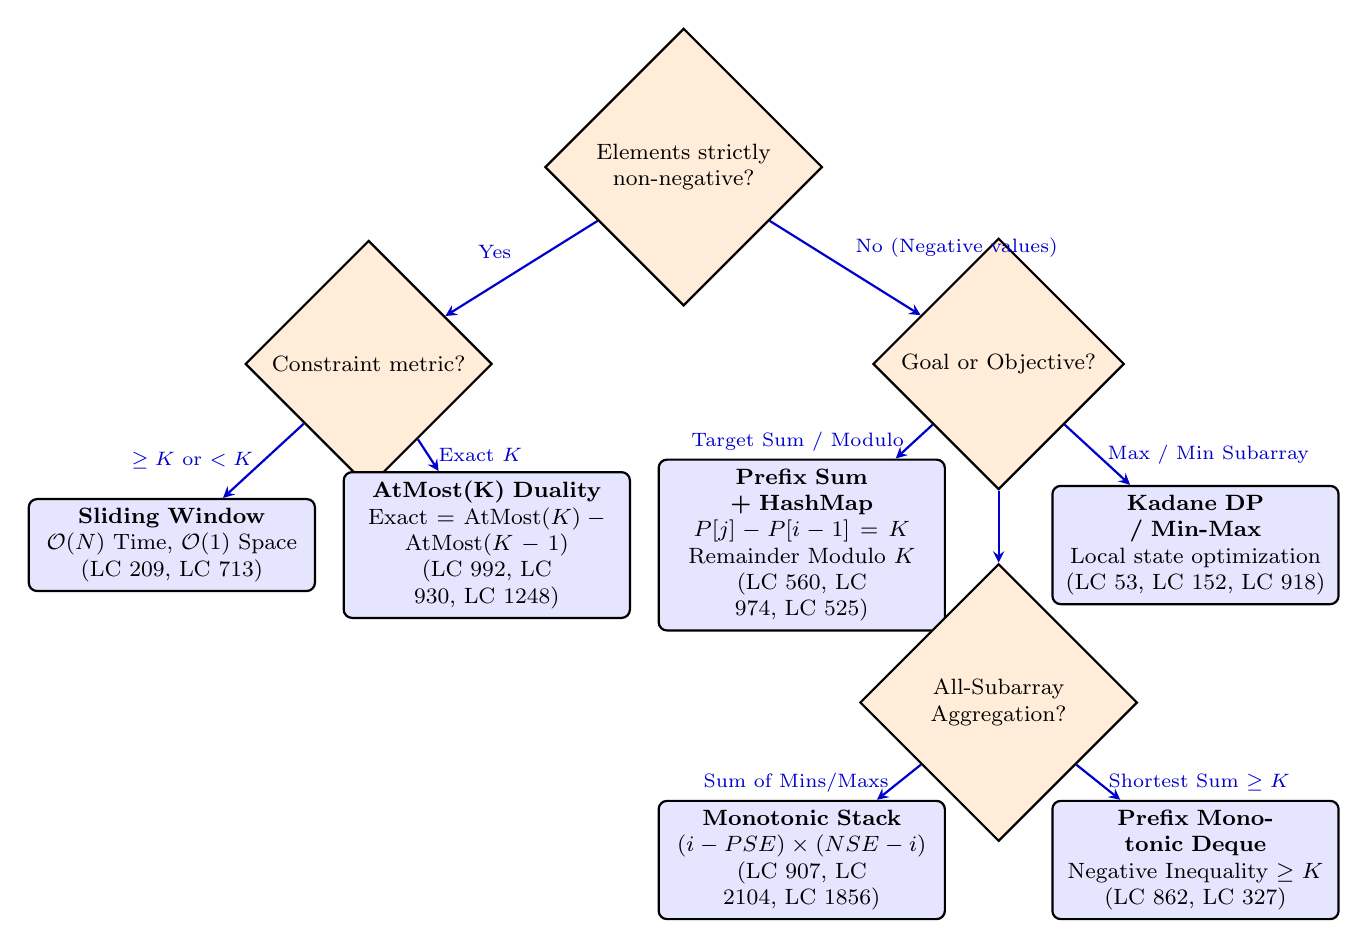
\begin{tikzpicture}[
    decision/.style={draw, diamond, thick, fill=orange!15, text width=2.8cm, align=center, inner sep=1pt, font=\footnotesize},
    block/.style={draw, rectangle, rounded corners=3pt, thick, fill=blue!10, text width=3.4cm, align=center, minimum height=0.8cm, font=\footnotesize},
    arr/.style={->, >=stealth, thick, color=blue!80!black}
]
    \node[decision] (d1) at (0, 0) {Elements strictly non-negative?};
    \node[decision] (d2) at (-4, -2.5) {Constraint metric?};
    \node[decision] (d3) at (4, -2.5) {Goal or Objective?};
    
    % Left branches (Non-negative)
    \node[block] (b1) at (-6.5, -4.8) {\textbf{Sliding Window}\\$\mathcal{O}(N)$ Time, $\mathcal{O}(1)$ Space\\(LC 209, LC 713)};
    \node[block] (b2) at (-2.5, -4.8) {\textbf{AtMost(K) Duality}\\$\text{Exact} = \text{AtMost}(K) - \text{AtMost}(K-1)$\\(LC 992, LC 930, LC 1248)};
    
    % Right branches (Mixed / Negative)
    \node[block] (b3) at (1.5, -4.8) {\textbf{Prefix Sum + HashMap}\\$P[j] - P[i-1] = K$\\Remainder Modulo $K$\\(LC 560, LC 974, LC 525)};
    \node[block] (b4) at (6.5, -4.8) {\textbf{Kadane DP / Min-Max}\\Local state optimization\\(LC 53, LC 152, LC 918)};
    
    \node[decision] (d4) at (4, -6.8) {All-Subarray Aggregation?};
    \node[block] (b5) at (1.5, -8.8) {\textbf{Monotonic Stack}\\$(i - PSE) \times (NSE - i)$\\(LC 907, LC 2104, LC 1856)};
    \node[block] (b6) at (6.5, -8.8) {\textbf{Prefix Monotonic Deque}\\Negative Inequality $\ge K$\\(LC 862, LC 327)};
    
    % Connections
    \draw[arr] (d1) -- node[above left, font=\scriptsize] {Yes} (d2);
    \draw[arr] (d1) -- node[above right, font=\scriptsize] {No (Negative values)} (d3);
    
    \draw[arr] (d2) -- node[left, font=\scriptsize] {$\ge K$ or $< K$} (b1);
    \draw[arr] (d2) -- node[right, font=\scriptsize] {Exact $K$} (b2);
    
    \draw[arr] (d3) -- node[left, font=\scriptsize] {Target Sum / Modulo} (b3);
    \draw[arr] (d3) -- node[right, font=\scriptsize] {Max / Min Subarray} (b4);
    
    \draw[arr] (d3) -- (d4);
    \draw[arr] (d4) -- node[left, font=\scriptsize] {Sum of Mins/Maxs} (b5);
    \draw[arr] (d4) -- node[right, font=\scriptsize] {Shortest Sum $\ge K$} (b6);
\end{tikzpicture}
\caption{The 10-Second LeetCode Subarray Problem Diagnostic Decision Flowchart.}
\label{fig:decision_flowchart}
\end{figure*}

\begin{table*}[htbp]
\caption{Comprehensive Master LeetCode Subarray Problem Taxonomy Matrix}
\label{tab:taxonomy_matrix}
\centering
\begin{tabular}{p{2.8cm}p{3.2cm}p{3.5cm}p{1.6cm}p{1.4cm}p{3.2cm}}
\toprule
\textbf{Paradigm} & \textbf{Core Input Condition} & \textbf{Target Metric / Constraint} & \textbf{Time} & \textbf{Space} & \textbf{Canonical LeetCode} \\
\midrule
\textbf{Prefix Hash Map} & Arbitrary Integers & Sum $= K$, Longest Zero Sum & $\mathcal{O}(N)$ & $\mathcal{O}(N)$ & LC 560, LC 525, LC 325 \\
\textbf{Prefix Remainder} & Modulo $K$ Division & Sum $\pmod K = 0$, Len $\ge 2$ & $\mathcal{O}(N)$ & $\mathcal{O}(K)$ & LC 974, LC 523, LC 1524 \\
\textbf{Sliding Window} & Non-negative $a_i \ge 0$ & Min Len Sum $\ge K$, Prod $< K$ & $\mathcal{O}(N)$ & $\mathcal{O}(1)$ & LC 209, LC 713, LC 1004 \\
\textbf{AtMost(K) Duality} & Monotonic Cardinality & Exactly $K$ Distinct Elements & $\mathcal{O}(N)$ & $\mathcal{O}(K)$ & LC 992, LC 930, LC 1248 \\
\textbf{Monotonic Deque} & Sliding Bounds & Max $-$ Min $\le$ Limit & $\mathcal{O}(N)$ & $\mathcal{O}(N)$ & LC 1438, LC 239 \\
\textbf{Kadane DP} & Mixed Real Numbers & Maximum / Minimum Subarray Sum & $\mathcal{O}(N)$ & $\mathcal{O}(1)$ & LC 53, LC 918 \\
\textbf{Dual Product DP} & Negative Factors & Maximum Subarray Product & $\mathcal{O}(N)$ & $\mathcal{O}(1)$ & LC 152 \\
\textbf{Subarray Modifications} & One Element Deletion & Maximum Subarray with 1 Delete & $\mathcal{O}(N)$ & $\mathcal{O}(1)$ & LC 1186, LC 1749 \\
\textbf{Monotonic Stack} & Element Contribution & Sum of Subarray Mins / Ranges & $\mathcal{O}(N)$ & $\mathcal{O}(N)$ & LC 907, LC 2104, LC 1856 \\
\textbf{Prefix Merge Sort} & Non-monotonic Ranges & Lower $\le \text{Sum} \le$ Upper & $\mathcal{O}(N \log N)$ & $\mathcal{O}(N)$ & LC 327 \\
\textbf{Prefix Deque} & Mixed Values & Shortest Subarray Sum $\ge K$ & $\mathcal{O}(N)$ & $\mathcal{O}(N)$ & LC 862 \\
\textbf{Bitwise Monotonic} & 32-bit Integers & Distinct Bitwise OR / XOR & $\mathcal{O}(30 N)$ & $\mathcal{O}(30 N)$ & LC 898, LC 1310, LC 2411 \\
\bottomrule
\end{tabular}
\end{table*}

\subsection{The 10-Second Problem Classification Framework}

When analyzing any new contiguous subarray problem in a technical interview:
\begin{enumerate}
    \item \textbf{Check Sign of Elements}:
    \begin{itemize}
        \item If elements are strictly non-negative $\implies$ \textbf{Two-Pointer Sliding Window} (\S\ref{sec:sliding-window}).
        \item If exact-$K$ count is requested $\implies$ \textbf{AtMost(K) Duality} (\S\ref{sec:atmost-duality}).
    \end{itemize}
    \item \textbf{Check Target Equality or Modulo Divisibility}:
    \begin{itemize}
        \item If searching for Sum $= K$ or Divisible by $K$ with negative numbers $\implies$ \textbf{Prefix-Sum Hash Map} (\S\ref{sec:prefix-hash}).
    \end{itemize}
    \item \textbf{Check Local State Extremum}:
    \begin{itemize}
        \item If seeking Maximum/Minimum sum or product of a single subarray $\implies$ \textbf{Kadane DP} (\S\ref{sec:dynamic-programming}).
    \end{itemize}
    \item \textbf{Check All-Subarray Aggregations}:
    \begin{itemize}
        \item If summing minimums, maximums, or min-products across \emph{all} subarrays $\implies$ \textbf{Monotonic Stack Contribution Principle} (\S\ref{sec:monotonic-stack}).
    \end{itemize}
    \item \textbf{Check Negative Prefixes with Inequalities}:
    \begin{itemize}
        \item If searching for shortest subarray with sum $\ge K$ or range sum bounds $\implies$ \textbf{Monotonic Deque on Prefixes} or \textbf{Merge-Sort Divide-and-Conquer} (\S\ref{sec:divide-conquer}).
    \end{itemize}
    \item \textbf{Check Bitwise Operations}:
    \begin{itemize}
        \item If evaluating bitwise OR or AND $\implies$ \textbf{30-Bit Monotonic Accumulation} (\S\ref{sec:bitwise}).
    \end{itemize}
\end{enumerate}

%% ============================================================
\section{Conclusion}
\label{sec:conclusion}

Contiguous subarray sequence optimization is one of the richest and most rigorously tested domains in algorithmic computer science. By shifting away from ad-hoc trial-and-error toward systematic paradigm classification, software engineers and researchers can immediately deduce optimal algorithms for any sequence bound. 

This paper has formalized the eight foundational subarray paradigms: from algebraic prefix hash transformations and monotonic two-pointer contractions, to set-theoretic AtMost dualities, Kadane dynamic programming, monotonic stack element contribution, and bitwise accumulation limits. Adherence to this unified theoretical framework guarantees optimal space-time asymptotic bounds and error-free implementation across competitive programming and mission-critical production systems.

\begin{thebibliography}{10}

\bibitem{bentley1984}
J.~Bentley, ``Programming Pearls: Algorithm Design Techniques,'' \emph{Communications of the ACM}, vol.~27, no.~9, pp.~865--873, 1984.

\bibitem{cormen2022}
T.~H.~Cormen, C.~E.~Leiserson, R.~L.~Rivest, and C.~Stein, \emph{Introduction to Algorithms}, 4th~ed.\hskip 1em plus 0.5em minus 0.4em\relax Cambridge, MA: MIT Press, 2022.

\bibitem{sedgewick2011}
R.~Sedgewick and K.~Wayne, \emph{Algorithms}, 4th~ed.\hskip 1em plus 0.5em minus 0.4em\relax Boston: Addison-Wesley, 2011.

\bibitem{leetcode2024}
LeetCode Engineering Team, ``Contiguous Subarray Problem Archive and Sequence Optimization Masterclass,'' 2024. [Online]. Available: \url{https://leetcode.com/problemset/all/}

\end{thebibliography}


\end{document}
